\documentclass[10pt,twocolumn]{article}

\usepackage[margin=0.75in]{geometry}
\usepackage{graphicx}
\usepackage{amsmath,amssymb}
\usepackage[T1]{fontenc}
\usepackage{lmodern}
\usepackage{booktabs}
\usepackage{hyperref}
\usepackage{xurl}
\usepackage{xcolor}
\usepackage{tikz}
\usetikzlibrary{arrows.meta,positioning,shapes.geometric,fit,calc,backgrounds}
\usepackage{enumitem}
\usepackage{abstract}
\usepackage{cite}
\usepackage{pifont}
\newcommand{\cmark}{\ding{51}}
\newcommand{\xmark}{\ding{55}}

\hypersetup{
  colorlinks=true,
  linkcolor=blue!60!black,
  citecolor=blue!60!black,
  urlcolor=blue!60!black
}

\setlength{\columnsep}{0.25in}
\setlength{\parskip}{0.3em}
\setlength{\parindent}{0pt}
\setlist{nosep,leftmargin=*}

\title{\textbf{Agents Unite: A Git-Native Proof-of-Trust Ledger\\for Distributed Financial Intelligence}}
\author{
  \textit{Open Financial Memory Initiative}\\
  \small github.com/rahiakil/agents-unite
}
\date{July 2026}

\begin{document}

\twocolumn[
\begin{@twocolumnfalse}
\maketitle
\begin{abstract}
\noindent
Autonomous large language model (LLM) agents can synthesize market sentiment, news flow, and technical context at scale, yet solo deployments face a dual constraint: \emph{token economics} that scale linearly with universe coverage, and \emph{temporal blind spots} that no single timezone can close. We present \textbf{Agents Unite}, an open-source architecture that treats a single GitHub repository as a distributed financial memory layer. Thousands of contributors each spend approximately \$0.05 of inference per day on one deterministically assigned ticker (versus roughly \$200--\$2{,}000 per day for a solo operator covering $\sim$4{,}000 U.S.\ names), submit structured reports via pull requests, and rely on verifier and consensus agents, coordinated by Raft-style leader election and proof-of-stake-inspired reputation weighting, to merge independent analyses into a canonical ledger. Unlike on-chain knowledge graphs, Agents Unite leverages existing Git workflows (CI validation, CODEOWNERS, immutable prompt hashes) as a lightweight consensus substrate. The resulting archive supports backtesting, retrieval-augmented generation (RAG), and longitudinal evaluation across equities, crypto, ETFs, and bonds at zero marginal inference cost for readers who fork the ledger. We argue this model reduces \emph{per-operator} token burden by four orders of magnitude, compounds history as the primary moat, and warrants a new class of open foundation, the \emph{Open Financial Memory Foundation}, analogous to the Apache Software Foundation but scoped to verifiable market intelligence.
\end{abstract}
\vspace{0.5em}
\end{@twocolumnfalse}
]

%=============================================================================
\section{Introduction}
%=============================================================================

Financial markets generate narrative, sentiment, and price information faster than any individual, human or agent, can absorb. Retail and institutional participants increasingly delegate synthesis to LLM agents, yet three structural failures persist:

\begin{enumerate}[label=\arabic*.]
  \item \textbf{Ephemeral memory.} Agent sessions discard work at termination; yesterday's NVDA analysis must be regenerated at full cost.
  \item \textbf{Budget exhaustion.} Covering $\sim$4{,}000 U.S.\ tickers daily with multi-step agentic research costs on the order of hundreds to thousands of dollars in API tokens per run when priced at July 2026 list rates (Table~\ref{tab:api-rates}) and a fixed report schema of $\sim$1{,}800 input / $\sim$700 output tokens plus harness overhead~\cite{openai-pricing,deepseek-pricing,architecture}.
  \item \textbf{Timezone asymmetry.} A cron job in Austin misses Tokyo open chatter, overnight Reddit spikes, and post-close filings.
\end{enumerate}

\textbf{Agents Unite}~\cite{agentsunite} reframes the problem: instead of one operator researching the entire market, \emph{the crowd researches one ticker each}. Assignment is deterministic (contributors cannot cherry-pick symbols), and outputs land in a versioned path \texttt{data/YYYY-MM-DD/TICKER/}. Git history becomes the asset: every belief is a commit, every merge is consensus, every fork is a derivative index.

This paper formalizes the architecture, draws precise analogies to distributed consensus and proof-of-stake systems, and outlines governance via an Apache-style foundation. Our thesis: \emph{the biggest moat is not the code; it is history.}

%=============================================================================
\section{Related Work}
%=============================================================================

We situate Agents Unite across verifiable multi-agent memory, crowd financial forecasts, and Git-shaped data versioning, an intersection none fully covers.

\paragraph{Decentralized AI agent infrastructure.}
OriginTrail anchors agent memory with on-chain proofs~\cite{origintrail}; Akashik uses peer-to-peer provenance chains~\cite{akashik}; HadAgent couples serving to proof-of-inference consensus~\cite{hadagent}; and PolyLink and VeriLLM emphasize verifiable inference quality~\cite{polylink,verillm}. Folklore shows that federated inference trees outperform single-node caches (Table~\ref{tab:federation})~\cite{folklore2026}. Agents Unite instead stores dated inference artifacts and sources in a searchable Git ledger. Consumers may still route generation through PolyLink/VeriLLM while reusing pooled ticker-day results. This trades cryptographic finality for Git-and-API deployability, with optional Phase~4 anchoring (Section~\ref{sec:git-substrate}).

\begin{table}[h]
\centering
\caption{Federated inference-tree sharing vs.\ single-node semantic cache (recall@1, $\leq$2\% false-accept; Folklore / BEIR)~\cite{folklore2026}.}
\label{tab:federation}
\scriptsize
\begin{tabular}{@{}lrrr@{}}
\toprule
\textbf{Corpus} & \textbf{Single-node} & \textbf{Federated trees} & \textbf{Gain} \\
\midrule
SciFact & 81.5\% & 98.2\% & +20.5\% \\
NFCorpus & 77.3\% & 97.6\% & +26.2\% \\
FiQA & 66.0\% & 94.5\% & +43.3\% \\
\bottomrule
\end{tabular}
\end{table}

\paragraph{Crowdsourced financial forecasting.}
Estimize and blind-submission follow-ons~\cite{estimize,jame2016,da2020} motivate crowd forecasts; DLT-Sentiment-News~\cite{dlt-sentiment} shows demand for open labels. Agents Unite differs in outputs, assignment, and draft isolation (Section~\ref{sec:estimize}).

\paragraph{Git-native agent and data patterns.}
lakeFS~\cite{lakefs}, Project Nessie~\cite{nessie}, and DuckLake~\cite{ducklake} provide Git-like data versioning by separating metadata from bulky objects. Agents Unite likewise keeps small, reviewable reports in Git while serving scale-out analytics from columnar snapshots (Section~\ref{sec:scalability}).

%=============================================================================
\section{Problem Formulation}
%=============================================================================

Let $T$ denote the ticker universe ($|T| \approx 4{,}000$), $C$ the daily active contributors, and $c$ the per-report inference cost. Table~\ref{tab:api-rates} lists July 2026 published per-million-token rates used throughout this paper. Combined with Agents Unite's fixed report schema ($\sim$1,800 input and $\sim$700 output tokens per report~\cite{architecture}), a single-ticker completion costs $\sim$\$0.001 on GPT-4o-mini~\cite{openai-pricing} or DeepSeek V4-Flash~\cite{deepseek-pricing}. With typical harness overhead (3--8 tool calls for source gathering), we estimate $c \approx \$0.05$ (range \$0.02--\$0.08 depending on model and adapter).

\begin{table}[h]
\centering
\caption{Recent published LLM API list prices (July 2026).}
\label{tab:api-rates}
\scriptsize
\begin{tabular}{@{}llrr@{}}
\toprule
\textbf{Model} & \textbf{Vendor page} & \textbf{Input \$/M} & \textbf{Output \$/M} \\
\midrule
GPT-4o-mini & OpenAI~\cite{openai-pricing} & 0.15 & 0.60 \\
DeepSeek V4-Flash & DeepSeek~\cite{deepseek-pricing} & 0.14 & 0.28 \\
Gemini 2.5 Flash-Lite & Google~\cite{gemini-pricing} & 0.10 & 0.40 \\
\bottomrule
\end{tabular}
\end{table}

Solo coverage cost is $O(|T| \cdot c)$: one operator researching the full universe spends $\sim$\$200--\$2{,}000/day (Figure~\ref{fig:costs}). Crowd coverage is $O(C \cdot c)$: each contributor spends only $c$, while readers fork the ledger at zero marginal inference cost. The economic gain is therefore \textbf{per-operator burden reduction}, not elimination of aggregate work:

\begin{itemize}
  \item \textbf{Temporal diversity}: agents in London, Tokyo, and Austin capture disjoint information windows;
  \item \textbf{Model diversity}: Claude, GPT, Gemini, DeepSeek, and local Ollama instances decorrelate hallucination errors~\cite{methods};
  \item \textbf{Focus diversity}: randomized slices (sentiment, news, social, trading) turn assignment collisions into complementary reports.
\end{itemize}

\subsection{Cost Model}

Table~\ref{tab:costmodel} derives the per-report estimate from published per-million-token rates. Solo scenarios multiply by $|T|$; the crowd scenario multiplies by one assignment per contributor.

\begin{table}[h]
\centering
\caption{Per-report cost model (July 2026 API rates).}
\label{tab:costmodel}
\scriptsize
\begin{tabular}{@{}lrrr@{}}
\toprule
\textbf{Component} & \textbf{Tokens} & \textbf{Rate} & \textbf{Cost} \\
\midrule
Input (canonical prompt) & 1,800 & \$0.15/M\cite{openai-pricing} & \$0.00027 \\
Output (structured report) & 700 & \$0.60/M\cite{openai-pricing} & \$0.00042 \\
Harness overhead ($\sim$5$\times$) & \multicolumn{2}{c}{tool calls, browsing} & \$0.0035 \\
\midrule
\textbf{Typical Agents Unite report} & \multicolumn{2}{c}{budget to premium harness} & \textbf{\$0.05} \\
\bottomrule
\end{tabular}
\end{table}

\begin{figure}[h]
\centering
\resizebox{\columnwidth}{!}{%
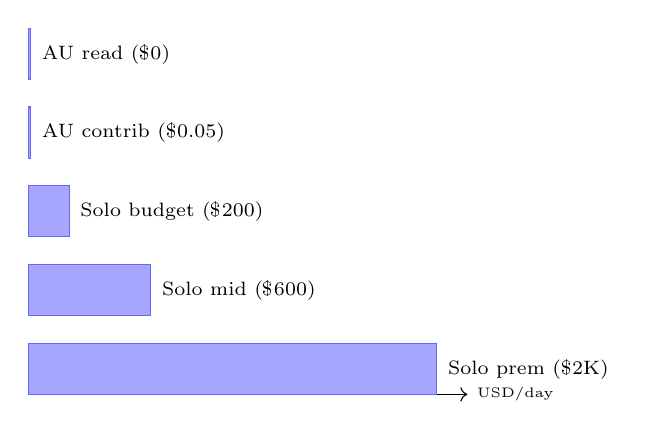
\begin{tikzpicture}[
  x=0.0026cm,
  bar/.style={fill=blue!35, draw=blue!60, line width=0.4pt},
  lbl/.style={font=\scriptsize, anchor=west}
]
  \draw[->] (0,0) -- (2150,0) node[right, font=\tiny] {USD/day};
  \foreach \y/\val/\name/\tag in {
    0/2000/Solo prem/\$2K,
    1/600/Solo mid/\$600,
    2/200/Solo budget/\$200,
    3/0.05/AU contrib/\$0.05,
    4/0/AU read/\$0} {
    \pgfmathsetmacro{\draww}{max(\val, 12)}
    \draw[bar] (0,\y) rectangle (\draww,\y+0.65);
    \node[lbl] at (\draww+8,\y+0.32) {\name\ (\tag)};
  }
\end{tikzpicture}%
}
\caption{Average daily inference cost by coverage model for a $\sim$4{,}000-ticker universe. \emph{AU contrib}: one Agents Unite contributor (\$0.05/day). \emph{AU read}: fork and consume existing reports (\$0). \emph{Solo budget/mid/prem}: single operator at \$0.05, \$0.15, and \$0.50 per ticker. Rates from Table~\ref{tab:api-rates}~\cite{openai-pricing,deepseek-pricing,gemini-pricing}.}
\label{fig:costs}
\end{figure}

\begin{table}[h]
\centering
\caption{Per-operator economics: solo vs.\ crowd (see Figure~\ref{fig:costs}).}
\label{tab:economics}
\small
\begin{tabular}{@{}lcc@{}}
\toprule
\textbf{Model} & \textbf{Daily cost} & \textbf{Coverage} \\
\midrule
Solo (budget, \$0.05/ticker) & $\sim$\$200 & $\sim$4{,}000 tickers \\
Solo (mid-tier, \$0.15/ticker) & $\sim$\$600 & $\sim$4{,}000 tickers \\
Solo (premium, \$0.50/ticker) & $\sim$\$2{,}000 & $\sim$4{,}000 tickers \\
\textbf{Agents Unite contributor} & \textbf{$\sim$\$0.05} & \textbf{1 ticker} \\
\textbf{Agents Unite reader} & \textbf{\$0} & \textbf{all history} \\
\bottomrule
\end{tabular}
\end{table}

\subsection{DIY Data vs.\ Contribute vs.\ Consume}
\label{sec:monetary}

Researchers choose among three paths:

\begin{enumerate}[label=\arabic*.]
  \item \textbf{DIY (solo).} One operator pays $O(|T|\cdot c)$ for full-universe research (Figure~\ref{fig:costs}, Table~\ref{tab:annual-stack}), plus vendor inputs.
  \item \textbf{Contribute.} Pay $\sim$\$0.05/day for one assigned ticker and merge into the shared ledger. The contributor's marginal cost buys coverage of \emph{their} assignment while unlocking read access to everyone else's history.
  \item \textbf{Consume (fork/read).} Pay \$0 inference to clone the archive and run backtests or RAG over accumulated \texttt{sentiment\_score} series. Price bars for return alignment still require a market-data API; the avoided cost is regenerating years of narrative/sentiment research.
\end{enumerate}

Agents Unite targets spend on \textbf{regenerated agent research} and \textbf{narrative alt-data}, not terminal price workflows (Table~\ref{tab:annual-stack}).

\begin{table}[h]
\centering
\caption{Indicative annual stack costs (2025--2026 published or surveyed averages).}
\label{tab:annual-stack}
\scriptsize
\begin{tabular}{@{}lp{3.6cm}r@{}}
\toprule
\textbf{Stack element} & \textbf{Source / basis} & \textbf{\$/yr} \\
\midrule
Bloomberg Terminal (1 seat) & Industry-reported 2026 list~\cite{bloomberg-cost} & $\sim$31{,}980 \\
Alt-data (avg.\ per dataset) & Neudata buyer survey~\cite{neudata2024} & $\sim$80{,}000 \\
Alt-data (avg.\ fund budget) & Neudata ($n{=}60$ buyers)~\cite{neudata2024} & $\sim$1.6M \\
Retail EOD API (Tiingo Power) & Vendor pricing~\cite{tiingo-pricing} & 360 \\
Intraday/history API (Polygon Adv.) & Vendor pricing~\cite{polygon-pricing} & 2{,}388 \\
Solo LLM full-universe (budget) & \$200/day $\times$ 365 (Table~\ref{tab:api-rates}) & $\sim$73{,}000 \\
Solo LLM full-universe (mid) & \$600/day $\times$ 365 & $\sim$219{,}000 \\
\textbf{AU contributor} & \$0.05/day $\times$ 365 & \textbf{$\sim$18} \\
\textbf{AU yes/no verify (est.)} & $\ll$\$0.01/check $\times$ 365 & \textbf{$\ll$\$4} \\
\textbf{AU reader (inference)} & Fork ledger & \textbf{0} \\
\bottomrule
\end{tabular}
\end{table}

\paragraph{Cheap verification: yes/no and cross-encoders.}
\label{sec:cheap-verify}
Full research agents are expensive because they browse, tool-call, and write long reports. Verifiers need not repeat that work. A practical cost reduction is \textbf{claim checking}: take a peer's posted report (or a single claim from it), retrieve the cited URL snippet, and ask a small model only for a binary judgment (``supported? yes/no'') with a short rationale. At GPT-4o-mini rates (Table~\ref{tab:api-rates}), a 400-token input / 20-token output check is on the order of \$10$^{-4}$ per claim, orders of magnitude below regenerating the report. Where even that is too heavy, \textbf{cross-encoder} rerankers and NLI models score (claim, evidence) pairs jointly without open-ended generation~\cite{nogueira2019,provenance2024}, enabling local CPU verification of source support and duplicate detection before a generative verifier is invoked. Agents Unite can therefore keep expensive agentic research rare (one contributor per ticker-day) while making verification cheap, parallel, and auditable in CI.

\paragraph{Backtesting savings from multiple angles.}
Backtests usually pay twice: for prices (Table~\ref{tab:market-data}) and narrative features. A shared ledger removes the second bill: fork tagged releases and \texttt{load\_reports.py} series instead of paying $365 \times |T| \times c$ to regenerate history or renewing alt-data feeds (Table~\ref{tab:annual-stack}). Recent reports remain searchable for RAG, and optional attestations~\cite{polylink,verillm} can re-verify them without re-crawling sources.

\begin{table}[h]
\centering
\caption{Recent published market-data API prices for backtesting labels (2026).}
\label{tab:market-data}
\scriptsize
\begin{tabular}{@{}llr@{}}
\toprule
\textbf{Product} & \textbf{Published rate} & \textbf{\$/yr} \\
\midrule
Tiingo Power (individual) & \$30/mo~\cite{tiingo-pricing} & 360 \\
Polygon Stocks Starter & \$29/mo~\cite{polygon-pricing} & 348 \\
Polygon Stocks Advanced & \$199/mo~\cite{polygon-pricing} & 2{,}388 \\
Bloomberg Terminal (1 seat) & \$31{,}980/yr~\cite{bloomberg-cost} & 31{,}980 \\
\bottomrule
\end{tabular}
\end{table}

\subsection{Precedent and Divergence from Estimize}
\label{sec:estimize}

Estimize established that open crowds can improve earnings-expectation measurement when contributor counts are large~\cite{jame2016,estimize}. Agents Unite shares the crowd premise but diverges on three axes: (i)~outputs are structured narrative reports with sources, not scalar EPS/revenue points; (ii)~ticker assignment is deterministic, so contributors cannot concentrate on popular names; (iii)~drafts are independent until merge, approximating Estimize's post-2015 blind design~\cite{da2020}. The product is therefore closer to a longitudinal belief census than to a competing IBES-style estimate feed.

\paragraph{Herding risk.}
Da and Huang~\cite{da2020} show that viewing peer forecasts causes contributors to underweight private information, improving individual accuracy while harming consensus. Agents Unite faces an analogous risk if early-merged reports, public leaderboards, or RAG over yesterday's consensus become focal points that later agents imitate. Schema validation and MAD outlier rejection blunt crude spam, but they do not by themselves restore informational independence when agents share training corpora, news wires, or retrieved context.

\paragraph{Proposed mitigation.}
We propose weighting consensus not only by contributor count or stake, but by \textbf{source diversity}: reports whose cited URL domains, modality slices (sentiment/news/social/trading), and model families are more orthogonal receive higher influence in the weighted median. Homogeneous clusters (many accounts citing the same wire story through the same harness) should not dominate simply because $n$ is large. Formal calibration of diversity weights, and whether diversity should enter before or after MAD filtering, is left to Phase~3--4 evaluation.

%=============================================================================
\section{System Architecture}
%=============================================================================

Figure~\ref{fig:arch} depicts the end-to-end pipeline. There is no central application server; \textbf{GitHub is the database}.

\begin{figure}[h]
\centering
\resizebox{\columnwidth}{!}{%
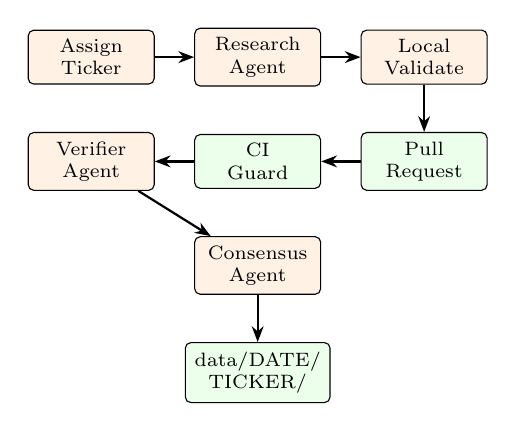
\begin{tikzpicture}[
  node distance=0.35cm and 0.5cm,
  box/.style={draw, rounded corners=2pt, minimum height=0.55cm, minimum width=1.6cm, align=center, font=\scriptsize, fill=blue!5},
  ghbox/.style={box, fill=green!8},
  agent/.style={box, fill=orange!10},
  arr/.style={-{Stealth[length=2mm]}, thick}
]
  \node[agent] (assign) {Assign\\Ticker};
  \node[agent, right=of assign] (research) {Research\\Agent};
  \node[agent, right=of research] (validate) {Local\\Validate};
  \node[ghbox, below=0.6cm of validate] (pr) {Pull\\Request};
  \node[ghbox, left=of pr] (ci) {CI\\Guard};
  \node[agent, left=of ci] (verify) {Verifier\\Agent};
  \node[agent, below=0.6cm of ci] (consensus) {Consensus\\Agent};
  \node[ghbox, below=0.6cm of consensus] (data) {data/DATE/\\TICKER/};

  \draw[arr] (assign) -- (research);
  \draw[arr] (research) -- (validate);
  \draw[arr] (validate) -- (pr);
  \draw[arr] (pr) -- (ci);
  \draw[arr] (ci) -- (verify);
  \draw[arr] (verify) -- (consensus);
  \draw[arr] (consensus) -- (data);
\end{tikzpicture}%
}
\caption{Distributed ingestion pipeline. Each contributor machine runs assignment, research, and validation locally; GitHub CI and peer agents provide trust anchors.}
\label{fig:arch}
\end{figure}

\subsection{Deterministic Assignment}

Ticker selection prevents manipulation:
\begin{equation}
  k = \text{SHA256}(\text{date} : \text{contributor\_hash}) \bmod |T|
\end{equation}
The assigned ticker is $T_k$ from a sorted, community-maintained universe file. Role selection uses a parallel hash lottery: $\sim$65\% research, $\sim$20\% verify, $\sim$15\% consensus~\cite{roles}.

\subsection{Report Schema}

Each artifact pair \texttt{report.*.md} + \texttt{sources.*.json} includes YAML frontmatter with \texttt{sentiment\_score} $\in [-1,1]$, \texttt{prompt\_hash}, and \texttt{github\_username}. Separating URLs into JSON keeps diffs readable and enables programmatic deduplication~\cite{architecture}.

%=============================================================================
\section{Consensus and Distributed Coordination}
%=============================================================================

A single agent report is noisy. Agents Unite implements a \textbf{three-stage consensus pipeline} inspired by Raft~\cite{raft} and proof-of-stake validator networks~\cite{ethereum-pos}.

\begin{figure}[h]
\centering
\resizebox{0.95\columnwidth}{!}{%
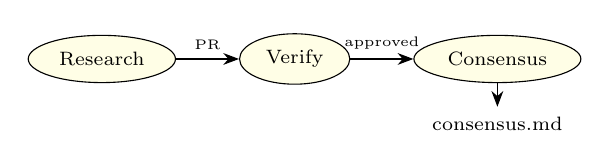
\begin{tikzpicture}[
  node distance=0.4cm,
  stage/.style={draw, ellipse, minimum width=1.4cm, minimum height=0.6cm, font=\scriptsize, fill=yellow!10},
  arr/.style={-{Stealth[length=2mm]}}
]
  \node[stage] (r) {Research};
  \node[stage, right=0.8cm of r] (v) {Verify};
  \node[stage, right=0.8cm of v] (c) {Consensus};
  \node[below=0.3cm of c, font=\scriptsize] (out) {consensus.md};

  \draw[arr] (r) -- node[above,font=\tiny]{PR} (v);
  \draw[arr] (v) -- node[above,font=\tiny]{approved} (c);
  \draw[arr] (c) -- (out);
\end{tikzpicture}%
}
\caption{Role pipeline: research $\rightarrow$ verify $\rightarrow$ consensus.}
\label{fig:pipeline}
\end{figure}

\subsection{Weighted Median Aggregation}

Given $n$ validated scores $\{x_i\}$:
\begin{enumerate}[label=(\roman*)]
  \item Compute median $m$ and MAD; reject outliers where $|x_i - m| > 2 \cdot \text{MAD}$.
  \item Compute weighted median with weights $w_i = \text{stake}_i \times \text{reputation}_i \times \text{recency}_i$.
  \item Assign confidence: \emph{high} if $n \geq 3$ and spread $\leq 0.4$; \emph{low} if $n = 1$~\cite{consensus}.
\end{enumerate}

Themes are \emph{not} forced into agreement; divergence is preserved in \texttt{consensus.md}. Verifier roles should prefer the cheap yes/no and cross-encoder path in Section~\ref{sec:cheap-verify} before spending a full research budget to re-derive the same memo.

\subsection{Raft Leader Election for Hourly Shards}

Phase~3 introduces hourly updates. Multiple writers to the same \texttt{(date, ticker, hour)} shard would cause Git conflicts. Agents Unite adopts \textbf{deterministic Raft-style leader election} without a blockchain:

\begin{equation}
  \text{leader} = \arg\min_{i} \text{SHA256}(\text{date} : \text{hour} : \text{ticker} : \text{hash}_i)
\end{equation}

Among contributors who submitted valid hourly reports, the minimum hash wins write authority for the consensus merge, analogous to Raft's single-leader principle~\cite{raft} but requiring no network partition protocol because GitHub serializes merges.

\begin{figure}[h]
\centering
\resizebox{\columnwidth}{!}{%
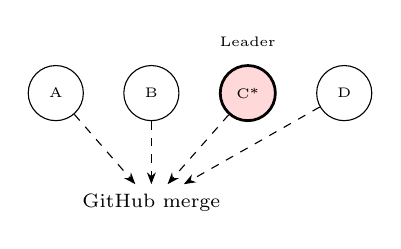
\begin{tikzpicture}[
  node distance=0.5cm,
  agent/.style={draw, circle, minimum size=0.7cm, font=\tiny},
  leader/.style={agent, fill=red!15, line width=1pt},
  arr/.style={-{Stealth[length=1.5mm]}, dashed}
]
  \node[agent] (a1) {A};
  \node[agent, right=of a1] (a2) {B};
  \node[leader, right=of a2] (a3) {C*};
  \node[agent, right=of a3] (a4) {D};
  \node[below=0.8cm of a2, font=\scriptsize] (gh) {GitHub merge};
  \draw[arr] (a1) -- (gh);
  \draw[arr] (a2) -- (gh);
  \draw[arr] (a3) -- (gh);
  \draw[arr] (a4) -- (gh);
  \node[above=0.1cm of a3, font=\tiny] {Leader};
\end{tikzpicture}%
}
\caption{Hourly shard: contributor C wins deterministic leader election and merges \texttt{consensus.md}.}
\label{fig:raft}
\end{figure}

\subsection{Proof-of-Stake Analogy}

Ethereum's proof-of-stake selects validators proportional to staked ETH~\cite{ethereum-pos}. Agents Unite's Phase~4 maps this to \textbf{reputation staking}:

\begin{itemize}
  \item \textbf{Stake} = accumulated accuracy vs.\ ex-post consensus and price outcomes;
  \item \textbf{Validators} = verifier agents with high merge approval rates;
  \item \textbf{Slashing} = reputation decay for rejected reports, fabricated URLs, or MAD outliers;
  \item \textbf{Rewards} = leaderboard visibility, weighted influence, eligibility for signal consumption.
\end{itemize}

No native token is required in Phase~1; reputation lives in \texttt{contributors/reputation.json}. Optional on-chain attestation layers (e.g., MINT Protocol~\cite{mint}) can anchor Merkle roots of daily snapshots without storing private data on-chain.

%=============================================================================
\section{Git as Consensus Substrate}
\label{sec:git-substrate}
%=============================================================================

Table~\ref{tab:git-blockchain} compares blockchain primitives to Git-native equivalents. Agents Unite occupies a middle ground: \emph{permissioned trust} via GitHub identity and CI, with \emph{permissionless read} via MIT license and fork.

\begin{table}[h]
\centering
\caption{Blockchain $\leftrightarrow$ Git mapping in Agents Unite.}
\label{tab:git-blockchain}
\scriptsize
\begin{tabular}{@{}ll@{}}
\toprule
\textbf{Blockchain} & \textbf{Agents Unite} \\
\midrule
Block & Commit \\
Validator set & Verifiers + CI \\
Consensus & Weighted median + merge \\
State trie & \texttt{data/DATE/TICKER/} \\
Smart contract & GitHub Actions workflows \\
Finality & Merged to \texttt{main} \\
\bottomrule
\end{tabular}
\end{table}

\subsection{Scalability and Operational Limits}
\label{sec:scalability}

Treating Git as a write-heavy database has a known failure mode. Package ecosystems that stored indexes in Git (crates.io's Cargo index, Homebrew taps, and nixpkgs-scale trees) eventually hit clone, fetch, and delta-resolution costs that forced sparse HTTP indexes, CDN JSON feeds, or channel tarballs~\cite{nesbitt2025}. A financial memory ledger that accumulates thousands of daily report files faces the same asymptotics: directory width, packfile growth, and CI clone time degrade before cryptographic consensus becomes the bottleneck. Shallow clones and sparse checkouts delay pain; they do not remove the need for a read path that is not ``git fetch the universe.''

Agents Unite therefore proposes a \textbf{hybrid storage path}: Git retains commits, PR review, CODEOWNERS, and per-report provenance (the collaboration substrate), while periodic \textbf{columnar snapshots} (Parquet/DuckDB-style exports keyed by date) serve analytics, RAG embedding jobs, and cold readers who need history without a full clone (mirroring the metadata/data split in lakeFS, Nessie, and DuckLake)~\cite{lakefs,nessie,ducklake}. Phase~4 Merkle roots of those snapshots can be attested on-chain (e.g., MINT-style anchoring~\cite{mint}) without moving private contributor data on-chain, connecting operational scale-out to the existing attestation roadmap. In this design, Git remains the system of record for contribution and dispute; snapshots are the system of record for bulk consumption.

%=============================================================================
\section{Foundation Governance}
\label{sec:foundation}
%=============================================================================

Sustainable open data requires neutral stewardship. We propose the \textbf{Open Financial Memory Foundation (OFMF)}, modeled on the Apache Software Foundation~\cite{apache}:

\begin{figure}[h]
\centering
\resizebox{0.9\columnwidth}{!}{%
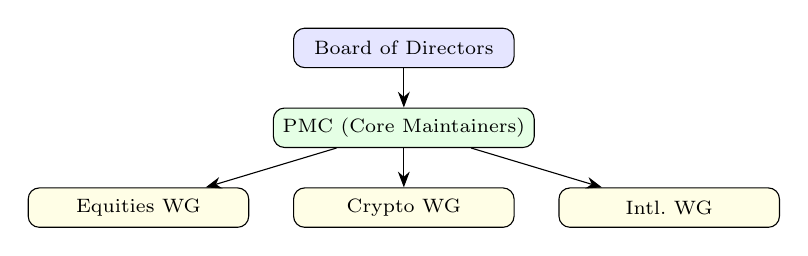
\begin{tikzpicture}[
  level/.style={draw, rounded corners, minimum width=2.8cm, minimum height=0.5cm, font=\scriptsize, align=center},
  arr/.style={-{Stealth[length=2mm]}}
]
  \node[level, fill=blue!10] (board) {Board of Directors};
  \node[level, fill=green!10, below=0.5cm of board] (pmc) {PMC (Core Maintainers)};
  \node[level, fill=yellow!10, below left=0.5cm and 0.3cm of pmc] (eq) {Equities WG};
  \node[level, fill=yellow!10, below=0.5cm of pmc] (crypto) {Crypto WG};
  \node[level, fill=yellow!10, below right=0.5cm and 0.3cm of pmc] (intl) {Intl.\ WG};
  \draw[arr] (board) -- (pmc);
  \draw[arr] (pmc) -- (eq);
  \draw[arr] (pmc) -- (crypto);
  \draw[arr] (pmc) -- (intl);
\end{tikzpicture}%
}
\caption{OFMF governance: Apache-style meritocracy with asset-class working groups.}
\label{fig:foundation}
\end{figure}

Key principles: (i)~individual merit over corporate affiliation; (ii)~immutable core (\texttt{scripts/}, \texttt{agents/}) protected by CODEOWNERS; (iii)~tagged dataset releases for reproducible backtests; (iv)~501(c)(3) structure to resist vendor capture.

%=============================================================================
\section{Adversarial Robustness and the Contribution Attack Surface}
%=============================================================================
% TODO(author): Manual review/rewrite before finalizing. Do not over-claim
% specific mitigations without author sign-off. This section flags attack
% surfaces; proposed defenses below are provisional discussion points only.

Open ingestion expands the attack surface beyond spam. Three Phase~1 gaps remain; proposed defenses below are provisional.

\paragraph{Indirect prompt injection via ingested sources.}
Research agents retrieve filings, news pages, and social threads. Adversaries can embed instructions in those documents so that retrieved content overrides the agent's intended task (indirect prompt injection)~\cite{greshake2023}. Schema checks and \texttt{prompt\_hash} bind the \emph{template}, not the retrieved payload. Verifier agents that re-read the same poisoned URLs may amplify rather than catch the attack. Candidate hardening directions include source sandboxing, explicit instruction/data delimiters, allowlisted domains, and verifier prompts that refuse to execute imperative language found in citations; none of these are asserted as sufficient without measurement.

\paragraph{Sybil and identity gaps in reputation.}
Phase~1 reputation lives in \texttt{contributors/reputation.json} keyed by GitHub identity. Cheap account creation, collusive rings, and recycled accuracy against a manipulable consensus remain open. MAD filters and merge-approval rates raise the cost of naive spam but do not constitute proof-of-human or stake-slashing. Claims about long-run Sybil resistance should await Phase~4 attestation design and measured attack simulations against the reputation update rule.

\paragraph{Limits of CI as the only gate.}
Contributor Guard and offline schema validation block malformed PRs and protected-path edits; they do not judge factual correctness, source authenticity, or coordinated narrative capture. CI is a necessary integrity gate, not a sufficient epistemic one. Human review, verifier diversity, and ex-post accuracy scoring remain load-bearing, and currently under-specified relative to the threat.

%=============================================================================
\section{Future Implications}
%=============================================================================

\textbf{For traders.} One forkable ledger replaces repeated full-market agent runs; consensus gating reduces single-model false positives (Section~\ref{sec:monetary}).

\textbf{For agent builders.} Canonical prompts, harness adapters, and verified merges create portable reputation.

\textbf{For society.} Open, versioned narrative features complement terminal-gated alt-data (Table~\ref{tab:annual-stack}).

\textbf{Risks.} Residual manipulation and poisoned sources (Section~9) require stronger attestation; outputs are structured observations, not investment advice.

\paragraph{Regulatory context.}
FINRA~\cite{finra2409} and SEC examination priorities~\cite{sec2025exams} apply when firms use generative AI in advisory workflows. Agents Unite is an MIT-licensed observation archive, not a registered adviser; commercial wrappers that personalize consensus scores inherit those duties. ``Observations, not advice'' labeling remains a first-order control.

At scale ($20{,}000$ installs $\times$ 15\% daily active $\approx$ 3{,}000 reports/day), Agents Unite approaches 75\% daily universe coverage, a density no solo agent achieves at any price.

%=============================================================================
\section{Agent Specialization and Analysis Modalities}
%=============================================================================

Role randomization splits each day's work into \textbf{complementary modalities}, so assignment collisions become ensemble coverage rather than redundant spend. \texttt{Sentiment}/\texttt{social} agents synthesize narrative mood from forums and social feeds into a bounded \texttt{sentiment\_score}, theme bullets, and attributed snippets. \texttt{Trading}/\texttt{full} agents ground those narratives in price, volume, range position, and catalyst tables. The \texttt{news} slice aggregates filings and headlines; verifiers cross-check cited numbers against source URLs, a lightweight peer analog to oracle checks. Figure~\ref{fig:modalities} shows how randomized focus merges into daily \texttt{consensus.md}.

\begin{figure}[h]
\centering
\resizebox{\columnwidth}{!}{%
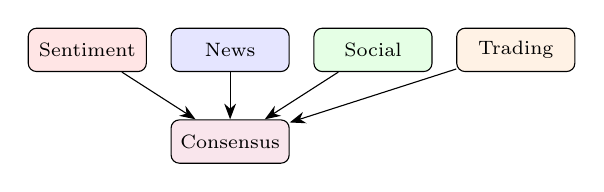
\begin{tikzpicture}[
  mod/.style={draw, rounded corners=3pt, minimum width=1.5cm, minimum height=0.55cm, font=\scriptsize, align=center},
  arr/.style={-{Stealth[length=2mm]}}
]
  \node[mod, fill=red!10] (s) {Sentiment};
  \node[mod, fill=blue!10, right=0.3cm of s] (n) {News};
  \node[mod, fill=green!10, right=0.3cm of n] (so) {Social};
  \node[mod, fill=orange!10, right=0.3cm of so] (t) {Trading};
  \node[mod, fill=purple!10, below=0.6cm of n] (c) {Consensus};
  \draw[arr] (s) -- (c);
  \draw[arr] (n) -- (c);
  \draw[arr] (so) -- (c);
  \draw[arr] (t) -- (c);
\end{tikzpicture}%
}
\caption{Complementary analysis modalities merge into daily \texttt{consensus.md}.}
\label{fig:modalities}
\end{figure}

%=============================================================================
\section{Asset Classes and Global Expansion}
%=============================================================================

Phase~1 seeds 291 U.S.\ equities, expanding via community PRs toward 4{,}000+. The same schema covers crypto (24/7 hourly shards under \texttt{tickers/crypto.json}), ETFs (macro layers above single names), bonds (yield-curve narratives favoring \texttt{news}/\texttt{trading} focus), and international symbols (LSE, TSE, HKEX) under OFMF working groups. Each class follows the Apache incubator pattern, prove schema fit, verifier coverage, and contributor density before graduation, preserving a \textbf{single canonical repository} and one Git history across asset classes.

%=============================================================================
\section{The Raft Census: Longitudinal Aggregation}
%=============================================================================

We introduce the term \textbf{Raft census} to describe the periodic aggregation of independent agent observations into consensus snapshots over calendar time. Unlike a one-shot sentiment poll, the census is:

\begin{enumerate}[label=\arabic*.]
  \item \textbf{Repeated}: daily (Phase~1), hourly (Phase~2+) observations per ticker;
  \item \textbf{Independent}: contributors cannot see others' drafts before submission;
  \item \textbf{Reconciled}: verifiers and consensus agents produce \texttt{consensus.md};
  \item \textbf{Immutable}: raw reports persist alongside canonical merges in Git history.
\end{enumerate}

This mirrors statistical sampling: each agent is an enumerator, verifiers are auditors, and consensus is official tabulation.

\subsection{Backtesting Methodology}

Quant researchers can construct sentiment factors from \texttt{consensus\_score} or raw \texttt{sentiment\_score} distributions:

\begin{enumerate}[label=(\alph*)]
  \item Load reports via \texttt{examples/load\_reports.py} for ticker $t$ and window $[t_0, t_1]$;
  \item Align scores to market close timestamps (configurable: UTC midnight or US close);
  \item Compute forward returns $r_{t+h}$ for horizons $h \in \{1, 5, 20\}$ days;
  \item Test monotonicity: do high-sentiment quintiles outperform low-sentiment quintiles?
  \item Attribute alpha to contributor subsets via \texttt{github\_username} for reputation calibration.
\end{enumerate}

Because every report includes \texttt{prompt\_hash} and source URLs, backtests are \textbf{reproducible}, a requirement absent from proprietary terminal feeds.

\subsection{RAG and LLM Downstream Queries}

The Phase~2 pipeline embeds reports into a searchable index and knowledge graph (\texttt{wiki/}). Example queries enabled by longitudinal memory:

\begin{itemize}
  \item ``Which bearish Reddit themes preceded NVDA's last twenty earnings misses?''
  \item ``How did consensus sentiment on regional banks evolve during March 2023?''
  \item ``Which contributors consistently led consensus by $\geq 3$ days?''
\end{itemize}

These queries run against crowd-collected history at fork cost (Section~\ref{sec:monetary}).

\subsection{Pending Empirical Evaluation}
\label{sec:pending-eval}

The following measurements are required before claiming production efficacy; \texttt{research/EXPERIMENTS.md} provides runbooks:

\begin{enumerate}[label=\arabic*.]
  \item \textbf{Sentiment factor backtest}: quintile spreads and IC for $h\in\{1,5,20\}$; needs $\geq$60 trading days and a price API (Table~\ref{tab:market-data}).
  \item \textbf{Ledger reuse vs.\ solo cache}: recall@1 at fixed false-accept on held-out ticker-day queries (Table~\ref{tab:federation}).
  \item \textbf{Verify cascade}: \$/decision and human agreement for re-research, yes/no, and cross-encoder NLI (Section~\ref{sec:cheap-verify}).
  \item \textbf{Source-diversity weights}: held-out calibration against equal-weight and stake-only aggregation (Section~\ref{sec:estimize}).
  \item \textbf{Adversarial probes}: injection and Sybil attack-success rates after CI and verifier checks; then revise Section~9.
\end{enumerate}

%=============================================================================
\section{Comparison with Related Architectures}
%=============================================================================

Table~\ref{tab:related} positions Agents Unite against contemporary decentralized AI memory and inference systems.

\begin{table}[h]
\centering
\caption{Agents Unite vs.\ related systems.}
\label{tab:related}
\scriptsize
\begin{tabular}{@{}lccc@{}}
\toprule
\textbf{System} & \textbf{Git-native} & \textbf{Financial} & \textbf{Live} \\
\midrule
OriginTrail DKG & \xmark & \xmark & \cmark \\
Akashik & \xmark & \xmark & \cmark \\
HadAgent & \xmark & \xmark & \cmark \\
Folklore & \xmark & \xmark & \cmark \\
DLT-Sentiment & \xmark & \cmark & \xmark \\
\textbf{Agents Unite} & \cmark & \cmark & \cmark \\
\bottomrule
\end{tabular}
\end{table}

Table~\ref{tab:related} summarizes the trade-off: Git-native deployability over on-chain finality (Section~2), with optional Phase~4 anchoring for tamper evidence.

%=============================================================================
\section{Conclusion}
%=============================================================================

Agents Unite demonstrates that \textbf{blockchain \emph{ideas} (consensus, stake-weighted trust, immutable history) need not require blockchain \emph{infrastructure}} when Git, CI, and open governance suffice. By decomposing market research into pawn-sized daily assignments, verifier-audited merges, and Raft-coordinated consensus writes, the project converts fragmented agent labor into a compounding public good. The moat is history; the mechanism is the crowd; the invitation is open.

%=============================================================================
\section*{Acknowledgments}
%=============================================================================
The Agents Unite open-source community and the maintainers of \url{github.com/rahiakil/agents-unite}.

\bibliographystyle{plain}
\bibliography{references}

\end{document}
